\documentclass[tikz,border=12pt]{standalone}
\usepackage{amsmath}
\usepackage{amssymb}
\usepackage{tikz}
\usetikzlibrary{calc,arrows.meta,decorations.pathmorphing,decorations.pathreplacing,positioning}

\begin{document}
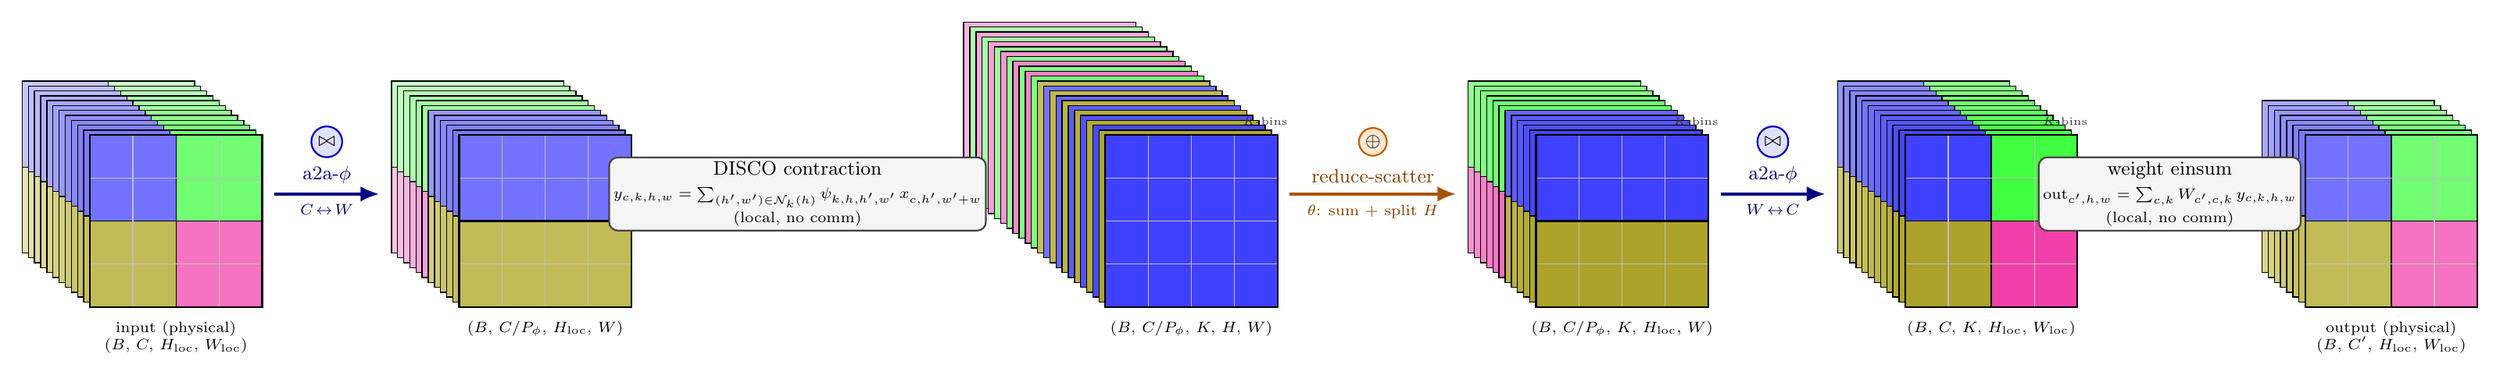
\begin{tikzpicture}[
  font=\sffamily,
  >=Latex,
  line width=0.5pt,
]

% ============================================================================
% Distributed DISCO conv — A2A variant, reduce-scatter on the polar H dim
%
% Code path (_distributed_disco_fwd_a2a in distributed_convolution_kernels.py):
%   (B, C, H_loc, W_loc)            input — physical, H×W sharded
%     ──[a2a azimuth: C ↔ W]──>     (B, C/P_phi, H_loc, W)
%   DISCO sparse contraction (K-expanded, local)
%                                   (B, C/P_phi, K, H_out, W)
%     ──[reduce-scatter polar (H)]──>   (B, C/P_phi, K, H_out_loc, W)
%     ──[a2a azimuth: W ↔ C]──>     (B, C, K, H_out_loc, W_out_loc)
%   weight einsum over (C, K)
%                                   (B, C', H_out_loc, W_out_loc)  output
%
% Communication: 2 a2as on the azimuth comm + 1 reduce_scatter on the polar
% comm. The DISCO contraction and the final weight einsum are both local.
% ============================================================================

% per-card stack offsets (channels go into the page, upper-left direction)
\def\dxIn{-0.10}\def\dyIn{0.08}

% ---------- helper: stacked yxgrid (channels = card stack on 2x2 spatial grid) ----
% args: cx, cy, halfwidth, n-cards, front-saturation, label
\newcommand{\yxstack}[6]{%
  \pgfmathtruncatemacro{\nm}{#4-1}%
  \foreach \k in {0,...,\nm}{%
    \pgfmathtruncatemacro{\j}{\nm-\k}%
    \pgfmathsetmacro{\ox}{#1 + \j*\dxIn}%
    \pgfmathsetmacro{\oy}{#2 + \j*\dyIn}%
    \pgfmathtruncatemacro{\sh}{#5 - \j*3}%
    \fill[blue!\sh!white,draw=black]    ({\ox-#3},{\oy})    rectangle ({\ox},{\oy+#3});%
    \fill[green!\sh!white,draw=black]   ({\ox},{\oy})       rectangle ({\ox+#3},{\oy+#3});%
    \fill[olive!\sh!white,draw=black]   ({\ox-#3},{\oy-#3}) rectangle ({\ox},{\oy});%
    \fill[magenta!\sh!white,draw=black] ({\ox},{\oy-#3})    rectangle ({\ox+#3},{\oy});%
  }%
  \foreach \i in {-1,1}{
    \draw[gray!50] ({#1+\i*#3/2},{#2-#3}) -- ({#1+\i*#3/2},{#2+#3});
    \draw[gray!50] ({#1-#3},{#2+\i*#3/2}) -- ({#1+#3},{#2+\i*#3/2});
  }
  \draw[thick] ({#1-#3},{#2-#3}) rectangle ({#1+#3},{#2+#3});
  \node[anchor=north,font=\scriptsize,align=center] at (#1,{#2-#3-0.10}) {#6};
}

% ---------- helper: row-uniform stack (rows colored polar, depth split azimuth) ----
% After the azimuth a2a, W is local per rank — each H row is owned by ONE
% polar rank, but along the channel (= depth) dim the data is split into
% TWO azimuth halves.
%   front half of stack  (channels owned by azimuth-0 ranks): blue (top) over olive (bottom)
%   back  half of stack  (channels owned by azimuth-1 ranks): green over magenta
%
% args: cx, cy, halfwidth, n-cards, front-saturation, label
\newcommand{\rowstack}[6]{%
  \pgfmathtruncatemacro{\nm}{#4-1}%
  \pgfmathtruncatemacro{\half}{#4/2}%
  \foreach \k in {0,...,\nm}{%
    \pgfmathtruncatemacro{\j}{\nm-\k}%
    \pgfmathsetmacro{\ox}{#1 + \j*\dxIn}%
    \pgfmathsetmacro{\oy}{#2 + \j*\dyIn}%
    \pgfmathtruncatemacro{\sh}{#5 - \j*3}%
    \ifnum\j<\half
      \fill[blue!\sh!white,draw=black]    ({\ox-#3},{\oy})    rectangle ({\ox+#3},{\oy+#3});%
      \fill[olive!\sh!white,draw=black]   ({\ox-#3},{\oy-#3}) rectangle ({\ox+#3},{\oy});%
    \else
      \fill[green!\sh!white,draw=black]   ({\ox-#3},{\oy})    rectangle ({\ox+#3},{\oy+#3});%
      \fill[magenta!\sh!white,draw=black] ({\ox-#3},{\oy-#3}) rectangle ({\ox+#3},{\oy});%
    \fi
  }%
  % subdivisions + thick border on FRONT-most card. Vertical centerline is
  % gray (W is local — no rank boundary there); horizontal is thick (polar
  % rank boundary).
  \foreach \i in {-1,1}{
    \draw[gray!50] ({#1+\i*#3/2},{#2-#3}) -- ({#1+\i*#3/2},{#2+#3});
    \draw[gray!50] ({#1-#3},{#2+\i*#3/2}) -- ({#1+#3},{#2+\i*#3/2});
  }
  \draw[gray!50] (#1,{#2-#3}) -- (#1,{#2+#3});
  \draw[thick] ({#1-#3},#2) -- ({#1+#3},#2);
  \draw[thick] ({#1-#3},{#2-#3}) rectangle ({#1+#3},{#2+#3});
  \node[anchor=north,font=\scriptsize,align=center] at (#1,{#2-#3-0.10}) {#6};
}

% ---------- helper: paired stack for B3 (partial-in-θ visualization) ----------
% Each rank holds the FULL H_out at B3 (each polar rank contributes
% partial values to every row; reduce-scatter will fold them). We render
% this as 2*Np cards — Np channel pairs of 2 — where within each pair the
% two cards carry the polar-0 and polar-1 partial contributions to the
% same channel. Colours match the rank palette from B1:
%   azimuth-0 channels (first \Np pairs):  (blue,  olive)   — polar 0, polar 1
%   azimuth-1 channels (last  \Np pairs):  (green, magenta) — polar 0, polar 1
% A subsequent reduce-scatter pairwise sums these and splits the rows,
% giving the consolidated \Np-card stack at B4.
%
% args: cx, cy, halfwidth, n-pairs, front-saturation, label
\newcommand{\paired}[6]{%
  \pgfmathtruncatemacro{\nTot}{2*#4-1}%
  \pgfmathtruncatemacro{\halfPairs}{#4/2}%
  \foreach \k in {0,...,\nTot}{%
    \pgfmathtruncatemacro{\j}{\nTot-\k}%
    \pgfmathsetmacro{\ox}{#1 + \j*\dxIn}%
    \pgfmathsetmacro{\oy}{#2 + \j*\dyIn}%
    \pgfmathtruncatemacro{\sh}{#5 - \j*2}%
    \pgfmathtruncatemacro{\pair}{\j/2}%        % which channel pair
    \pgfmathtruncatemacro{\pol}{mod(\j,2)}%    % 0 = polar-0 partial, 1 = polar-1 partial
    \ifnum\pair<\halfPairs
      \ifnum\pol=0
        \def\cardcol{blue}%
      \else
        \def\cardcol{olive}%
      \fi
    \else
      \ifnum\pol=0
        \def\cardcol{green}%
      \else
        \def\cardcol{magenta}%
      \fi
    \fi
    \fill[\cardcol!\sh!white,draw=black] ({\ox-#3},{\oy-#3}) rectangle ({\ox+#3},{\oy+#3});%
  }%
  % Full 4x4 gridlines: the 2 quarter lines in each direction, plus the
  % two centerlines. The centerlines are GRAY (not thick) because at B3
  % each rank holds the full H and full W — those midlines no longer mark
  % a rank boundary, they're just completing the cell grid for visual
  % continuity with the other blocks.
  \foreach \i in {-1,1}{
    \draw[gray!50] ({#1+\i*#3/2},{#2-#3}) -- ({#1+\i*#3/2},{#2+#3});
    \draw[gray!50] ({#1-#3},{#2+\i*#3/2}) -- ({#1+#3},{#2+\i*#3/2});
  }
  \draw[gray!50] (#1,{#2-#3}) -- (#1,{#2+#3});
  \draw[gray!50] ({#1-#3},#2) -- ({#1+#3},#2);
  \draw[thick] ({#1-#3},{#2-#3}) rectangle ({#1+#3},{#2+#3});
  \node[anchor=north,font=\scriptsize,align=center] at (#1,{#2-#3-0.10}) {#6};
}

% ============================================================================
% LAYOUT — six square blocks. Same blue/green/olive/magenta rank palette
% throughout — what changes per stage is the on-card layout (2x2 quadrants
% vs. row-uniform stripes vs. polar-paired partials) plus the saturation,
% which bumps up at the DISCO contraction (entering the K-expanded regime)
% and drops back at the weight einsum (collapses K and projects C → C').
% ============================================================================
\def\halfw{1.4}
\pgfmathsetmacro{\cY}{(11*\dyIn)/2}   % arrow baseline (visual mid of 12-card stack)

% channel-stack depths — input C and output C' differ.
\def\Nin{12}                          % input C channel cards
\def\NinH{24}                         % B3: full H_out (× 2 vs H_loc) ⇒ doubled depth
\def\Nout{8}                          % output C' channel cards (post weight einsum)

\def\satPhys{55}                      % saturation in the physical regime
\def\satK{75}                         % saturation in the K-expanded regime

% --------- B1: physical input (H×W sharded, C local) ---------
\yxstack{0}{0}{\halfw}{\Nin}{\satPhys}{input (physical)\\$(B,\,C,\,H_\text{loc},\,W_\text{loc})$};

% --------- B2: after a2a #1 — W local, C split azimuth ---------
% Rows uniform across W; channel dim now split-azimuth into stack depth
% (front cards = azimuth 0, back = azimuth 1).
\def\xB{6.0}
\rowstack{\xB}{0}{\halfw}{\Nin}{\satPhys}{$(B,\,C/P_\phi,\,H_\text{loc},\,W)$};

% --------- B3: after DISCO contraction — K-expanded, full H_out (partial in θ) ---------
% Each rank now holds the FULL H_out (partial in θ). The stack DOUBLES
% from \Nin → 2*\Nin, organised as \Nin channel PAIRS — within each pair
% the two cards carry the polar-0 and polar-1 partial contributions to
% the same channel (colours = the H-split palette from B1: blue+olive
% for azimuth-0 channels, green+magenta for azimuth-1). Reduce-scatter
% will fold each pair into one card and split rows → consolidated B4.
% K-bins tag drawn above.
\def\xC{16.5}
\paired{\xC}{0}{\halfw}{\Nin}{\satK}{$(B,\,C/P_\phi,\,K,\,H,\,W)$};
\node[font=\tiny,gray!40!black]
  at ({\xC+\halfw-0.20},{\halfw+0.22}) {$K$-bins};

% --------- B4: after reduce-scatter on polar H — H_out_loc, K still expanded ---------
% Sharding now matches B2 again (H split polar, W local) — RS has folded
% the partial-θ contributions into proper H_out_loc shards, so the stack
% depth shrinks back to \Nin. K still present, saturation held at the
% K-expanded level.
\def\xD{23.5}
\rowstack{\xD}{0}{\halfw}{\Nin}{\satK}{$(B,\,C/P_\phi,\,K,\,H_\text{loc},\,W)$};
\node[font=\tiny,gray!40!black]
  at ({\xD+\halfw-0.20},{\halfw+0.22}) {$K$-bins};

% --------- B5: after a2a #2 — C local, H_out_loc + W_out_loc both sharded ---------
% Back to 2x2 quadrants (both H and W sharded again, C gathered into
% local per rank). Saturation still K-bumped — the K dim is alive until
% the weight einsum.
\def\xE{29.5}
\yxstack{\xE}{0}{\halfw}{\Nin}{\satK}{$(B,\,C,\,K,\,H_\text{loc},\,W_\text{loc})$};
\node[font=\tiny,gray!40!black]
  at ({\xE+\halfw-0.20},{\halfw+0.22}) {$K$-bins};

% --------- B6: physical output (after weight einsum, K collapsed, C → C') ---------
% Channel stack THINS from Nin to Nout to reflect C → C' (also K folded
% in). Saturation drops back to the physical level.
\def\xF{36.0}
\yxstack{\xF}{0}{\halfw}{\Nout}{\satPhys}{output (physical)\\$(B,\,C',\,H_\text{loc},\,W_\text{loc})$};

% ============================================================================
% ARROWS + LABELS
% Each B1-B5 block: 12-card stack at (cx,0); back-card left = cx-halfw-1.1.
% B6: 8-card stack; back-card left = cx-halfw-0.7.
% ============================================================================
\def\xPad{0.20}
\pgfmathsetmacro{\xRightOff}{\halfw+\xPad}                   % +1.6 from block centre
\pgfmathsetmacro{\xLeftOffIn}{\halfw+(\Nin-1)*0.10+\xPad}    % -2.7 for N=12
\pgfmathsetmacro{\xLeftOffInH}{\halfw+(\NinH-1)*0.10+\xPad}  % -3.9 for N=24 (B3)
\pgfmathsetmacro{\xLeftOffOut}{\halfw+(\Nout-1)*0.10+\xPad}  % -2.3 for N=8

% --- A1: input → B2 (a2a azimuth) ---
\coordinate (a1s) at ({0+\xRightOff},\cY);
\coordinate (a1e) at ({\xB-\xLeftOffIn},\cY);
\draw[-{Latex[length=3mm,width=2.5mm]},very thick,blue!50!black] (a1s) -- (a1e);
\node[font=\small,anchor=south,blue!40!black]
  at ($(a1s)!0.5!(a1e)+(0,0.05)$) {a2a-$\phi$};
\node[font=\scriptsize,anchor=north,blue!40!black,align=center]
  at ($(a1s)!0.5!(a1e)+(0,-0.05)$) {$C\!\leftrightarrow\!W$};
\node[draw=blue!75!black,thick,fill=blue!12,circle,inner sep=2pt,font=\small] (i1)
  at ($(a1s)!0.5!(a1e)+(0,0.85)$) {$\bowtie$};

% --- A2: B2 → B3 (DISCO contraction — local). B3 has the deeper N=24
% stack, so we land on its back-card left edge via \xLeftOffInH.
\coordinate (a2s) at ({\xB+\xRightOff},\cY);
\coordinate (a2e) at ({\xC-\xLeftOffInH},\cY);
\draw[-{Latex[length=3mm,width=2.5mm]},very thick,gray!55!black] (a2s) -- (a2e);
\node[draw=gray!55!black,thick,fill=gray!8,rounded corners,
      minimum width=42mm,minimum height=11mm,align=center,font=\small,inner sep=2pt]
  (disco) at ($(a2s)!0.5!(a2e)$)
  {DISCO contraction\\
   {\scriptsize $y_{c,k,h,w}=\sum_{(h',w')\in\mathcal{N}_k(h)} \psi_{k,h,h',w'}\,x_{c,h',w'+w}$}\\
   {\scriptsize (local, no comm)}};

% --- A3: B3 → B4 (reduce-scatter on polar H) ---
\coordinate (a3s) at ({\xC+\xRightOff},\cY);
\coordinate (a3e) at ({\xD-\xLeftOffIn},\cY);
\draw[-{Latex[length=3mm,width=2.5mm]},very thick,orange!65!black] (a3s) -- (a3e);
\node[font=\small,anchor=south,orange!50!black]
  at ($(a3s)!0.5!(a3e)+(0,0.05)$) {reduce-scatter};
\node[font=\scriptsize,anchor=north,orange!50!black,align=center]
  at ($(a3s)!0.5!(a3e)+(0,-0.05)$) {$\theta$: sum + split $H$};
\node[draw=orange!75!black,thick,fill=orange!18,circle,inner sep=1.2pt,font=\small] (rs)
  at ($(a3s)!0.5!(a3e)+(0,0.85)$) {$\oplus$};

% --- A4: B4 → B5 (a2a #2 azimuth, W ↔ C) ---
\coordinate (a4s) at ({\xD+\xRightOff},\cY);
\coordinate (a4e) at ({\xE-\xLeftOffIn},\cY);
\draw[-{Latex[length=3mm,width=2.5mm]},very thick,blue!50!black] (a4s) -- (a4e);
\node[font=\small,anchor=south,blue!40!black]
  at ($(a4s)!0.5!(a4e)+(0,0.05)$) {a2a-$\phi$};
\node[font=\scriptsize,anchor=north,blue!40!black,align=center]
  at ($(a4s)!0.5!(a4e)+(0,-0.05)$) {$W\!\leftrightarrow\!C$};
\node[draw=blue!75!black,thick,fill=blue!12,circle,inner sep=2pt,font=\small] (i2)
  at ($(a4s)!0.5!(a4e)+(0,0.85)$) {$\bowtie$};

% --- A5: B5 → B6 (weight einsum — local; K collapse + C → C') ---
\coordinate (a5s) at ({\xE+\xRightOff},\cY);
\coordinate (a5e) at ({\xF-\xLeftOffOut},\cY);
\draw[-{Latex[length=3mm,width=2.5mm]},very thick,gray!55!black] (a5s) -- (a5e);
\node[draw=gray!55!black,thick,fill=gray!8,rounded corners,
      minimum width=36mm,minimum height=11mm,align=center,font=\small,inner sep=2pt]
  (mix) at ($(a5s)!0.5!(a5e)$)
  {weight einsum\\
   {\scriptsize $\mathrm{out}_{c',h,w}=\sum_{c,k} W_{c',c,k}\,y_{c,k,h,w}$}\\
   {\scriptsize (local, no comm)}};

% ============================================================================
% Title (commented — uncomment if you want a header)
% ============================================================================
%\node[font=\large\bfseries,anchor=south,gray!25!black]
%  at ({(\xB+\xE)/2}, 3.4)
%  {Distributed DISCO conv (A2A)};
%
%\node[font=\scriptsize,anchor=south,align=center,gray!45!black,text width=13cm]
%  at ({(\xB+\xE)/2}, 3.0)
%  {\textit{2 a2as on $\phi$ + 1 reduce-scatter on $\theta$;\ \ DISCO contraction and weight einsum are both local.}};

\end{tikzpicture}
\end{document}
